\documentclass[xcolor=svgnames]{beamer}
\usetheme{Boadilla}

\usepackage[utf8]{inputenc}
\usepackage[T1]{fontenc}
\usepackage{lmodern}
\usepackage[whole]{bxcjkjatype}
\usepackage[backend=biber]{biblatex}
\addbibresource{octave.bib}
\usepackage{mathtools}
\usepackage{multimedia}
\usepackage{siunitx}
\usepackage{pifont}
\usepackage{tikz}
\newcommand*\colorcheck[1]{%
  \expandafter\newcommand\csname #1check\endcsname{\textcolor{#1}{\ding{52}}}%
}
\colorcheck{green}

\title[GNU Octave]{Scientific programming with GNU Octave
  \includegraphics[width=1.5em]{res/images/octave-logo-1024.png}
}
\author[Kai T. Ohlhus]{
  オールフス カイトーベン \\
  OHLHUS, Kai Torben}
\institute[TWCU]{
  理学研究科 \\
  Graduate School of Science \\
  東京女子大学 \\
  Tokyo Woman's Christian University}
\date{November 22, 2019}
\titlegraphic{
\vfill
\hfill\includegraphics[height=1em]{res/images/cc-by-sa}
}

\begin{document}

{
\usebackgroundtemplate{
  \vbox to \paperheight{\vfil\hbox to \paperwidth{\hfil
  \tikz\node[opacity=0.15] {
  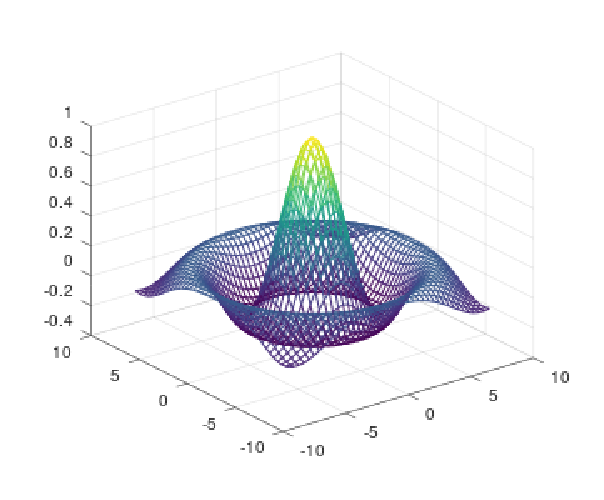
\includegraphics[width=0.8\paperwidth]{res/images/example-mesh}
  };
  \hfil}\vfil}
}
\frame{\titlepage}
}


\section{About GNU Octave}
\frame{\tableofcontents}
\begin{frame}{What is GNU Octave? - A community perspective.}
\begin{center}
\includegraphics[width=0.8\textwidth]{res/libreoffice/octave_community}
\end{center}
\end{frame}



\begin{frame}{What is GNU Octave? - A technical perspective.}
\vspace*{-1em}
\begin{center}
\includegraphics[width=0.8\textwidth]{res/libreoffice/octave_structure}
\end{center}
\end{frame}



\begin{frame}{Why GNU \textbf{"Octave"}?}

\begin{itemize}
\itemsep2em
\item
About \textbf{1992} \textbf{\color{DarkBlue}John W. Eaton (jwe)}
starts development\\[0.5em]
\begin{itemize}
\itemsep1em
\item
since then in total about \textbf{440 contributors}
\item
currently about \textbf{10-14 active developers}\footnote{Contributions to Octave core within last (two) month(s). \\
$\quad$ \texttt{\tiny hg log -r"date('>2019-11-24')" | grep user | sort | uniq}}
\end{itemize}

\item
Named after \textbf{\color{DarkBlue}Octave Levenspiel} (1926-2017)\\[0.5em]
\begin{itemize}
\itemsep1em
\item
former professor of jwe
\item
famous for quick back-of-the-envelope calculations
\end{itemize}
\end{itemize}
\end{frame}


\begin{frame}{Why \textbf{"GNU"} Octave?}

\begin{itemize}
\itemsep1.5em
\item
"GNU" (recursive: "GNU's Not Unix!")
Octave since \textbf{1997} (version 2.0.6)

\item
Shared
\textbf{philosophy}\footnote{\url{https://www.gnu.org/philosophy/free-sw.html}}
with the \textit{GNU project}
(\textit{Free Software Foundation}, FSF):\\[0.5em]

\begin{itemize}
\itemsep1em
\item
"[...] the freedom to run, copy, distribute, study, change
and improve the software. [...]"
\item
"[...] 'free' as in 'free speech,' not as in 'free beer'. [...]"

\end{itemize}

\item
Using \textbf{infrastructure} (e.g. code hosting and bug tracking)\\[0.5em]

\begin{itemize}
\item
SourceForge (1999), GitHub (2008), ...
\end{itemize}

\item
\textbf{Sponsorship} "Working Together for Free Software Fund"
\end{itemize}
\end{frame}



\section{Installation}
\frame{\tableofcontents[currentsection]}
\begin{frame}{Installing GNU Octave on MS Windows 10 (1/8)}
\begin{center}
\includegraphics[width=0.8\textwidth]{res/ms_windows/win_octave_gui.png}
\end{center}
\end{frame}



\begin{frame}{Installing GNU Octave on MS Windows 10 (2/8)}
\begin{center}
\url{https://www.octave.org/download}
\end{center}
\begin{columns}
\begin{column}{0.5\textwidth}
\includegraphics[width=0.9\textwidth]{res/ms_windows/win_download_cropped.png}
\end{column}
\begin{column}{0.4\textwidth}
\begin{itemize}
\itemsep0.8em
\item
\textbf{w32}: 32-bit systems (very old or embedded devices)

\item
\textbf{w64}: 64-bit systems \greencheck

\item
\textbf{w64-64}: 64-bit systems with \textbf{large} main memory
$2^{32} \times 8 \,Bytes = 32 \,GB$\\[0.5em]

Working with dense double matrices with $400,000 \times 100,000$ entries
($\approx 298 \,GB$) \textbf{need} this.
\end{itemize}
\end{column}
\end{columns}
\end{frame}



\begin{frame}{Installing GNU Octave on MS Windows 10 (3/8)}
\begin{columns}
\begin{column}{0.5\textwidth}
\textbf{Ignore} Java warning:
\begin{itemize}
\item
Octave works perfectly without Java.

\item
Octave's Java interface might not work properly.
\end{itemize}

\vspace*{2em}

\textbf{Choose:}
\begin{itemize}
\item
{\color{DarkBlue}OpenBLAS} (usually faster)

{\footnotesize \url{https://www.openblas.net/}}

\item
{\color{DarkBlue}Reference BLAS}

{\footnotesize \url{https://www.netlib.org/blas/}}
\end{itemize}
\end{column}
\begin{column}{0.4\textwidth}
\includegraphics[width=\textwidth]{res/ms_windows/win_install_java_warning.png}
\\[1em]
\includegraphics[width=\textwidth]{res/ms_windows/win_install_blas.png}
\end{column}
\end{columns}
\end{frame}



\begin{frame}{Installing GNU Octave on MS Windows 10 (4/8)}
\begin{itemize}
\item
As usual: desktop icons (left) and start menu entries (right).
\end{itemize}
\begin{columns}
\begin{column}{0.4\textwidth}
\includegraphics[width=0.6\textwidth]{res/ms_windows/win_install_desktop_icons.png}
\end{column}
\begin{column}{0.4\textwidth}
\includegraphics[width=0.8\textwidth]{res/ms_windows/win_install_startmenu_icons.png}
\end{column}
\end{columns}
\begin{itemize}
\item
Start
\begin{itemize}
\item
\textbf{command-line interface (CLI)}
\item
\textbf{graphical user interface (GUI)}
\end{itemize}
\end{itemize}
\end{frame}



\begin{frame}{Installing GNU Octave on MS Windows 10 (5/8)}
\begin{center}
\includegraphics[width=0.9\textwidth]{res/ms_windows/win_octave_cli_plot.png}
\end{center}
\end{frame}



\begin{frame}{Installing GNU Octave on MS Windows 10 (6/8)}
\begin{center}
\includegraphics[width=0.9\textwidth]{res/ms_windows/win_octave_gui_plot.png}
\end{center}
\end{frame}



\begin{frame}{Installing GNU Octave on MS Windows 10 (7/8)}
\begin{itemize}
\item
Many \textbf{\color{DarkBlue}Octave Forge} packages precompiled
as part of the installer.
\item
No need to download them, just \textbf{load} them.

$\quad\rightarrow$ \texttt{pkg list}
$\qquad\quad\;\rightarrow$ \texttt{pkg load io}
\end{itemize}
\begin{center}
\includegraphics[width=0.6\textwidth]{res/ms_windows/win_octave_packages.png}
\end{center}
\vspace*{-0.8em}
\texttt{C:\textbackslash Octave\textbackslash Octave-5.1.0.0\textbackslash
  mingw64\textbackslash share\textbackslash octave\textbackslash packages}
\end{frame}



\begin{frame}{Installing GNU Octave on MS Windows 10 (8/8)}
\begin{columns}
\begin{column}{0.3\textwidth}
\includegraphics[width=\textwidth]{res/ms_windows/win_octave_settings.png}
\end{column}
\begin{column}{0.6\textwidth}
\begin{itemize}
\itemsep2em
\item
Setting files in User's home directory.

e.g. \texttt{C:\textbackslash Users\textbackslash kai}

\item
Delete them if GUI is not starting.

\item
Use/start Octave without GUI from other programs, see
\texttt{\small C:\textbackslash Octave\textbackslash
Octave-5.1.0.0\textbackslash
octave.vbs}
\end{itemize}
\end{column}
\end{columns}
\end{frame}
\begin{frame}{Setup for this meeting}
\begin{itemize}
\itemsep1em
\item
Please find all material for the "hands on" sessions at:

{\color{DarkBlue}
\url{https://github.com/octave-de/octave_slides/releases/tag/2019-12-24}
}

\item
In general \textbf{Jupyter notebooks} are provided to the audience
to investigate several use cases of GNU Octave.

\item
For the best experience of the "hands on" sessions,
please bring your own laptop with Internet connection and the following setup
({\color{red}
\href{https://github.com/octave-de/octave_slides/releases/tag/2019-12-24/setup.pdf}{setup.pdf}}):

\begin{itemize}
\itemsep1em
\item
GNU Octave (see next slide)
\item
JupyterLab
({\color{DarkBlue}\url{https://jupyterlab.readthedocs.io/en/stable/}})
\item
octave\_kernel
({\color{DarkBlue}\url{https://github.com/Calysto/octave_kernel}})
\end{itemize}
\end{itemize}
\end{frame}


\begin{frame}{General installation steps on several systems}
$\rightarrow$ \url{https://wiki.octave.org/Installation}
\bigskip
\begin{columns}
\begin{column}{0.4\textwidth}
\includegraphics[width=\textwidth]{res/images/octave_wiki_install_linux}
\end{column}
\begin{column}{0.4\textwidth}
\includegraphics[width=0.42\textwidth]{res/images/octave_wiki_install_commercial}

\includegraphics[width=0.6\textwidth]{res/images/octave_wiki_install_other}
\bigskip\bigskip\bigskip
\end{column}
\end{columns}
\end{frame}


\section{Using Octave (Demos)}
\frame{\tableofcontents[currentsection]}
\begin{frame}{Using Octave (Demos)}
\begin{itemize}
\itemsep2em
\item
\textbf{\color{DarkBlue}\texttt{data\_io\_visualization.ipynb}}
\begin{itemize}
\item
Data I/O
\item
Plotting
\end{itemize}

\item
\textbf{\color{DarkBlue}\texttt{optimizing\_m\_code.ipynb}}

\item
\textbf{\color{DarkBlue}\texttt{fortran.ipynb}}
\begin{itemize}
\item
Octave and C/C++/Fortran
\end{itemize}

\item
In the GUI
\begin{itemize}
\item
Debugging and Profiling
\end{itemize}
\end{itemize}
\end{frame}



\section{Development}
\frame{\tableofcontents[currentsection]}
\begin{frame}{Octave development in a Nutshell}
\begin{center}
\includegraphics[width=0.85\textwidth]{res/libreoffice/dev_workflow}
\end{center}
\end{frame}

\begin{frame}{Some selected ongoing efforts}

From mailing-lists
and {\color{DarkBlue}\url{https://wiki.octave.org/Projects}}:\\[1em]
\begin{itemize}
\itemsep1em
\item
Octave.app for macOS
\hfill{\scriptsize\color{DarkBlue} \url{https://octave-app.org}}
\item
Python interface
\hfill{\scriptsize\color{DarkBlue} \url{https://wiki.octave.org/Pythonic}}
\item
Tabular data structure
\hfill{\scriptsize\color{DarkBlue}
\url{https://github.com/apjanke/octave-tablicious}}
\item
Improved \texttt{pkg} tool
\hfill{\scriptsize\color{DarkBlue}
\url{https://github.com/apjanke/octave-packajoozle}}
\item
Better graphics and \texttt{classdef} support
\item
Improved GUI terminal widget
\item
...
\end{itemize}
\end{frame}


\section{Reporting Bugs and Getting Help}
\frame{\tableofcontents[currentsection]}
\begin{frame}{Reporting problems, ask for help (1/2)}
Please, first look at:
\bigskip
\begin{itemize}
\item
\itemsep1em
{\color{DarkBlue}\url{https://octave.1599824.n4.nabble.com}}
(mailing-list archive)
\item
{\color{DarkBlue}\url{http://bugs.octave.org}} (bug tracker)
\end{itemize}
\bigskip\bigskip
\begin{columns}
\begin{column}{0.4\textwidth}
\includegraphics[width=\textwidth]{res/images/nabble_mailing_list_search}
\end{column}
\begin{column}{0.6\textwidth}
\includegraphics[width=\textwidth]{res/images/savannah_bug_search}
\end{column}
\end{columns}
\end{frame}



\begin{frame}{Reporting problems, ask for help (2/2)}
\begin{columns}
\begin{column}{0.55\textwidth}
\includegraphics[width=0.9\textwidth]{res/images/savannah_bug_report}
\end{column}
\begin{column}{0.45\textwidth}
In case of any problems\\[0.8em]

\textbf{We are happy to help you!}\\[1em]
\begin{itemize}
\itemsep1em
\item
Write us:
\begin{itemize}
\itemsep1em
\item
{\color{DarkBlue}\url{help@octave.org}}
\item
IRC freenode (\#octave)
\end{itemize}
\item
Report us:
\begin{itemize}
\item
{\color{DarkBlue}\url{http://bugs.octave.org}}
\end{itemize}
\end{itemize}
\bigskip\bigskip
\end{column}
\end{columns}
\end{frame}



\section{Wrapping up}
\frame{\tableofcontents[currentsection]}
\begin{frame}{Wrapping up: What is GNU Octave?}
\begin{center}
\includegraphics[width=0.8\textwidth]{res/libreoffice/octave_community}
\end{center}
\end{frame}



\begin{frame}{Wrapping up: What is GNU Octave?}
\begin{itemize}
\item
Todo
\end{itemize}
\end{frame}



\begin{frame}
\begin{center}
\textbf{\Large Thank you for your attention!}

\bigskip

\textbf{\Large Q+A?}
\end{center}
\vfill
Slides and sources available at:
{\color{DarkBlue}\url{https://github.com/octave-de/octave_slides}}
\end{frame}


\end{document}
